\documentclass[times, utf8, zavrsni]{fer}
\usepackage{booktabs}
\usepackage{xcolor}
\usepackage{listings}
\usepackage{subcaption}

\lstdefinelanguage{Dockerfile}
{
  morekeywords={FROM, RUN, CMD, LABEL, MAINTAINER, EXPOSE, ENV, ADD, COPY,
    ENTRYPOINT, VOLUME, USER, WORKDIR, ARG, ONBUILD, STOPSIGNAL, HEALTHCHECK,
    SHELL},
  morecomment=[l]{\#},
  morestring=[b]"
}

\lstset{
    columns=flexible,
    keepspaces=true,
    showstringspaces=false,
    basicstyle=\tiny\ttfamily,
    commentstyle=\color{gray},
    keywordstyle=\color{purple},
    stringstyle=\color{green}
}


\begin{document}

% TODO: Navedite broj rada.
\thesisnumber{1207}

% TODO: Navedite naslov rada.
\title{Detekcija kibernetičkih napada i zaštita vanjskih sustava u kontekstu mamaca za
operatora prijenosnog sustava}

% TODO: Navedite vaše ime i prezime.
\author{Filip Šimičević}

\maketitle

% Ispis stranice s napomenom o umetanju izvornika rada. Uklonite naredbu \izvornik ako želite izbaciti tu stranicu.
\izvornik

% Dodavanje zahvale ili prazne stranice. Ako ne želite dodati zahvalu, naredbu ostavite radi prazne stranice.
\zahvala{}

\tableofcontents

\chapter{Uvod}
Zbog napretka tehnologije pa tako i željom za pronalaženje boljih riješenja po pitanju održavanja električne mreže, operatori prijenosnih sustava se svakim danom razvijaju i koriste razne nove tehnologije i automatizacijske procese kako bi nam olakšali svakodnevni život. Međutim, time su uveli nove ranjivosti i rizike, posebno u području kibernetičke sigurnosti. Kibernetički napadi postali su značajna briga, prijeteći integritetu, dostupnosti i povjerljivosti osjetljivih informacija i kritične infrastrukture. Kako bi se osigurali od materijalne ili fizičke štete operatori prijenosnih sustava trebaju primjenjivati veće mjere zaštite i koristiti suvremene tehnologije koje pružaju optimalna riješenja za takve probleme. U ovom radu sam detaljno obradio zaštitu mamcima koji su samo jedan od temelja sigurnosti koji bi trebali biti implementirani u ovim sustavima. Implementacijom ovog modula, napadači mogu naići na naizgled ranjivu mašinu koja se lako podvija njihovm zahtjevima no u stvarnosti im u najmanju ruku trošimo vrijeme koje bi koristili za napad na pravi sustav. Također možemo prikupljati dragocjene podatke o samoj osobi koja stoji iza malicijoznih radnji.

\chapter{Operatori prijenosnih sustava}

\section{Definicija}
Uloge OPS-a na tržištu električne energije uključuju upravljanje sigurnošću elektroenergetskog sustava u stvarnom vremenu i koordinaciju ponude i potražnje za električnom energijom čime se izbjegavaju fluktuacije u frekvenciji ili prekidi u opskrbi. 
Svi OPS-ovi dužni su održavati stalnu (iz sekunde u sekundu) ravnotežu između opskrbe električnom energijom iz elektrana i potražnje potrošača, te također osigurati osiguranje rezervi koje će omogućiti iznenadne nepredviđene situacije. Većinom je državla vlasnik takvih institucija. [\cite{tso}]

\section{Industrijski upravljači sustavi}
Industrijski upravljački sustav (engl. ICS) zajednički je pojam za različite vrste upravljačkih sustava i pridružene instrumente koji uključuju uređaje, sustave, mreže i kontrole koji se koriste za rad i/ili automatizaciju industrijskih procesa. Ovisno o industriji, svaki ICS funkcionira drugačije i dizajniran je za učinkovito elektroničko upravljanje zadacima. Danas se uređaji i protokoli koji se koriste u ICS-u koriste u gotovo svim industrijama i kritičnim infrastrukturama, kao što su proizvodnja, transport, energija i obrada vode. Najpopularniji tipovi ICS-a su SCADA sustavi i distribuirani sustavi upravljanja. [\cite{ics-def}]

\section{PLC Sustavi}

PLC je programabilni logički kontroler, odnosno industrijsko računalo sastavljeno od memorije, procesora, industrijskog ulaza i izlaza, pri čemu ulaz nije tipkovnica, već tipke i sklopke, odnosno razne vrste pretvarača ili senzora. PLC se uglavnom koristi u industriji kao osnovna komponenta sustava automatizacije upravljanja, a njegovi programi ili algoritmi mogu se lako mijenjati za brza rješenja i aplikacije. Dio su brojnih strojeva i procesa u industriji.
 PLC je digitalno računalo u kojem se program izvršava u petlji koja se sastoji od tri faze:
\begin{itemize}
\item{čitanje ulazne varijable}
\item{Izvođenje programskog koda}
\item{iIspis rezultata logičke operacije na izlazu}
\end{itemize}

Programi se pohranjuju u unutarnju memoriju uređaja čak i kada je napajanje isključeno. Dizajniran je za teške uvjete rada i otporan je na vibracije, promjene temperature i električne smetnje.[\cite{plc2}]
\subsection{programski jezici}
Za kodiranje PLC-ova koristi se 5 programksih jezika:
\begin{itemize}
\item{ljestvičasta logika}
\item{dijagram funkcijskih blokova (FBD)}
\item{strukturirani tekst (ST)}
\item{popis uputa (IL)}
\item{sekvencijalna funkcionalna shema (SFC)}
\end{itemize} [ \cite{plc}]

\section{SCADA Sustavi}

\subsection{Arhitektura}
tipični SCADA sustav sastoji se od hijerarhije sljedećih komponenti:
\begin{itemize}
\item{pretvornika i aktuatora}
\item{RTU (eng. Remote Terminal Unit)}
\item{komunikacijske mreže}
\item{centralne stanice}
\end{itemize} [\cite{scada-arh}]
Ove komponente čine kontrolnu petlju nadzorne povratne sprege u SCADA sustavu.
\begin{figure}[htb]
\centering
\includegraphics[width=14cm]{slike/scada-arch.png}
\caption{Zaštita OPS sustava  [\cite{scada-thesis2}]}
\label{fig:scada-arch}
\end{figure}


\subsubsection{pretvornici i aktuatori}
Pretvornik i aktuator predstavljaju početak lanca. Imaju električnu ili mehaničku vezu s procesom koji promatramo. Zadatak pretvornika je praćenje vrijednosti tlaka, protoka, temperature, brzine itd. te prijenos podataka o izmjerenom trenutnom stanju u RTU u analognom ili digitalnom obliku. Aktuator prima informacije od RTU-a, kao što je zatvaranje ili otvaranje ventila.
[\cite{scada-thesis}]

\subsubsection{RTU (eng. Remote Terminal Unit)}
RTU-ovi su povezani s pretvornicima i aktuatorima i obično pohranjuju kontrolne parametre koje im senzori pošalju i izvršavaju programe koji izravno kontroliraju parametre električne energije. Stoga postoji stalna razmjena podataka i kontrola između RTU-ova, pretvornika i aktuatora koje tvore lokalnu povratnu kontrolnu petlju. RTU čuvaju prikupljene informacije u svojoj memoriji i čekaju zahtjev od MTU za prijenos podataka.
[\cite{scada-thesis}]

\subsubsection{komunikacijska mreža}
Komunikacijska mreža povezuje sve komponente ovog sustava i omogućuje im komunikaciju. Također omogućuje praćenje podataka u stvarnom vremenu.
[\cite{scada-thesis}]

\subsubsection{centralna stanica (MTU)}
MTU je glavna upravljačka jedinica koja sadrži stvarni SCADA softver, obično je povezana s mnogim RTU-ovim putem komunikacijskih kanala. MTU inicira sve komunikacije između RTU-a i sebe. Također je zadatak MTU-a da komunicira s drugim perifernim uređajima u objektu poput monitora, pisača, korporativne mreže i drugih informacijskih sustava. 

MTU provjerava RTU-ove u redovitim vremenskim intervalima kako bi pročitao podatke koje je prikupio RTU. Informacije o MTU prikazuju se na korisničkom sučelju kako bi se ljudskim operaterima omogućilo praćenje i upravljanje procesima pametne mreže. 

Operateri na MTU-u imaju mogućnost poništiti/promijeniti/nadjačati kritične radne parametre u bilo kojem dijelu SCADA mreže kada je to potrebno.

[\cite{scada-thesis}]

\subsection{Ranjvosti SCADA Sustava}
SCADA sustavi sami po sebi nisu građeni da zaštite podatke s kojima rukuju. Njihova zadaća je očitavanje senzora te određene akcije povratnom spregom ovisno o grani primjene. Potrebne su implementacije dodatnih zaštita kako bi se osigurali svi sigurnosni zahtjevi. 

Većina ovih sustava koriste Linux ili Windows operativni sustav koji imaju već globalno poznate ranjivosti koje napadači mogu iskoristiti. 
Još veći rizik se javlja ako su verzije operativnog sustava koji se koristi zastarjele.

Također se u ovakvim sustavim treba obratiti pozornost na protokole koji se koriste u mreži. Ako ti modeli ne sadržavaju adekvatnu kontrolu pristupa to sa sobom donosi skup problema koji potencionalno nisu ni riješivi sa zakrpama (engl. "patch"). Najčešće korišteni protokoli su MODBUS and DNP3. Većina komponenata može komunicirati MODBUS protokolom i zato se često izabire dok DNP3 nudi veći standard zaštite.

Ovi izolirani sustavi se spajaju na globalnu mrežu kako bi operatorima omogućili spajanje i time dali uvid u komponente, njihova očitanja, upravljanje i sl. no to stvara i priliku za potencionalne napadače da dobiju pristup sistemu.
[\cite{scada-thesis}]

\section{Najčešće prijetnje}
Operatori prijenosnih sustava uz SCADA sustave koriste i razne druge koji omogućuju npr. povezivanje zaposlenika unutar kompanije, isplaćivanje plaće, bilježenje radnog vremena. Oni također mogu biti kompromitirani i pružati vektor napada u sustav. Ako napadač dobije pristup na računalo nekog zaposlenika koji ima potrebne ovlasti za pristupanje nekom kritičnom dijelu sustava, cijeli taj blok postaje potencijonalno kompromitiran. 
ENISA je predstavila glavne kategorije prijetnji za 2020. kako slijedi: zlonamjerni softver, napadi temeljeni na webu/web aplikacijama, društveni inženjering (phishing, spam), distribuirano uskraćivanje usluge, krađa identiteta, povreda podataka, unutarnja prijetnja, botnet, fizička manipulacija i šteta , curenje informacija, ransomware, kibernetičko ratovanje/špijunaža i kriptovaluta.
 [\cite{tso-vuln}]
\section{Zaštite koje se primjenjuju}
\begin{figure}[htb]
\centering
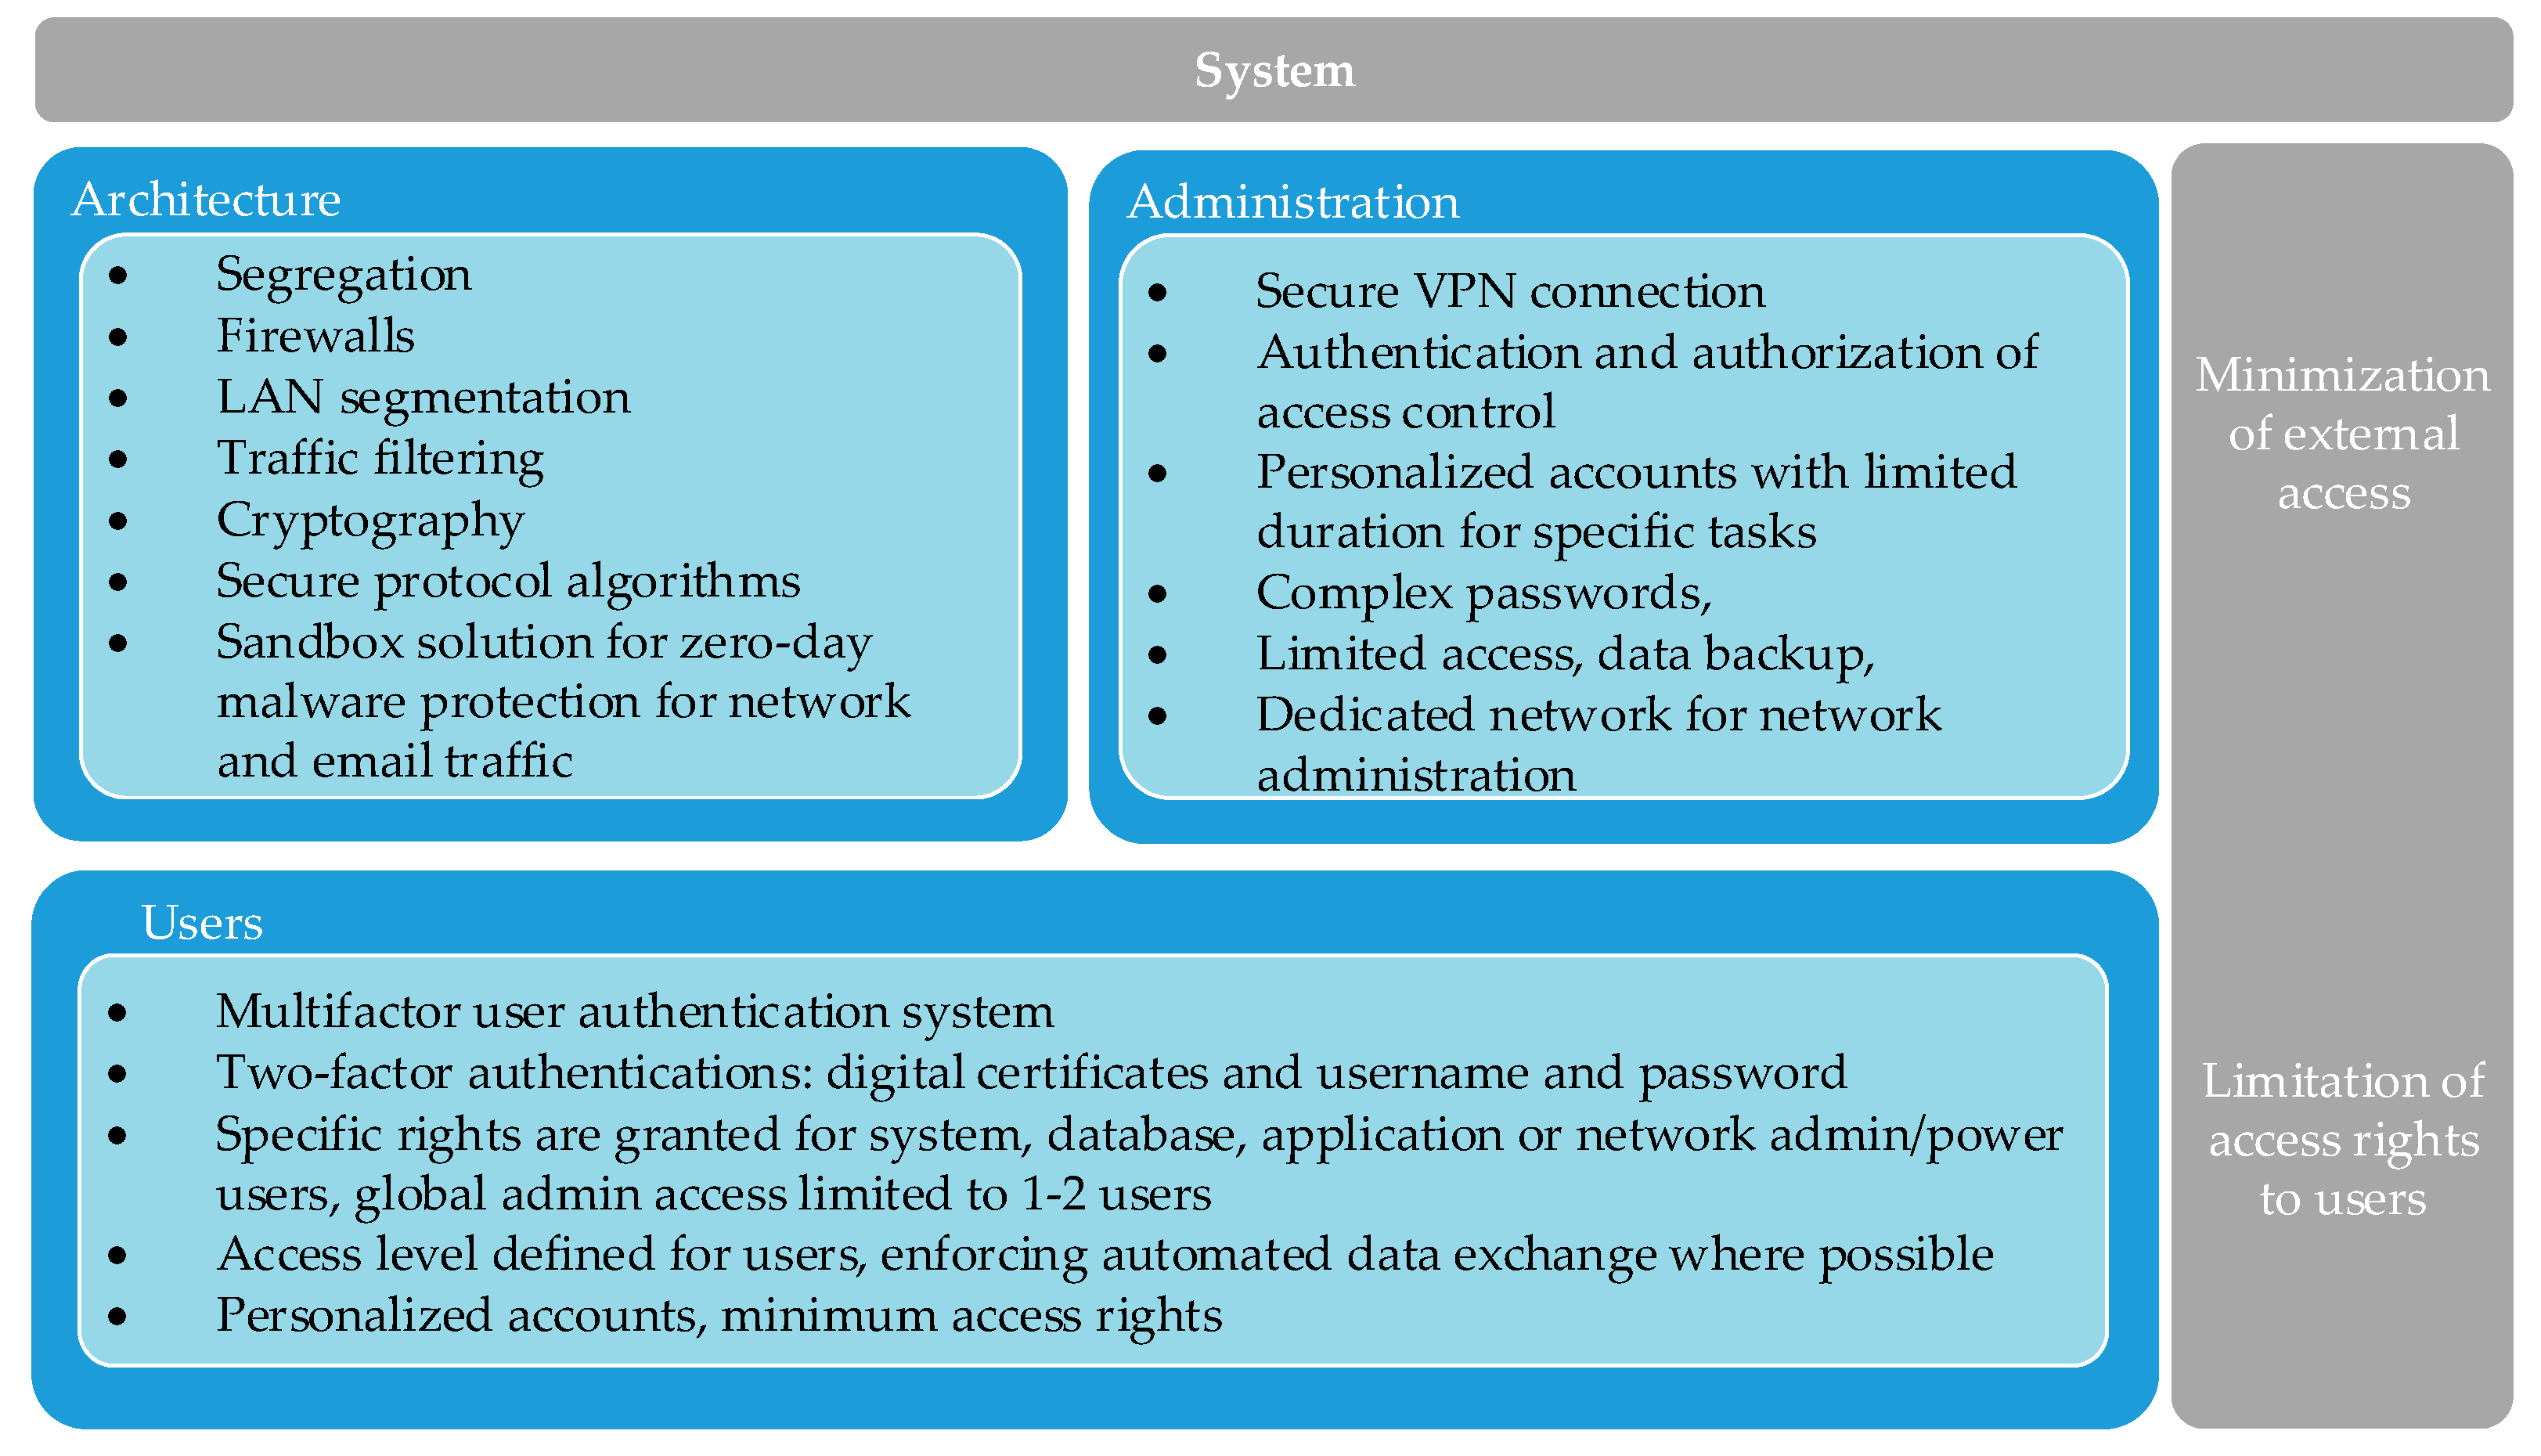
\includegraphics[width=14cm]{slike/Zastita-tso-sustava.png}
\caption{Zaštita OPS sustava  [\cite{tso-vuln}]}
\label{fig:Zastita-ops-sustava}
\end{figure}
Implementacija segregacije i vatrozida su među najčešćim mjerama zaštite zajedno s filtriranjem prometa i antivirusnim programima. Administrativni poslovi na važnim infrastrukturnim objektima obavljaju se putem računa koji nametaju određena ograničenja (ograničenje trajanja vremena, zaštita lozinkom, ograničenja pristupa). Uobičajeni pristup je implementacija višefaktorskog autentifikacije korisnika, ali također se koriste i specifična prava pristupa za korisnike koji obavljaju zadatke u kritičnim okruženjima (definicija različitih razina pristupa za različite vrste korisnika, personalizirani računi, minimalna prava za pristup). Korisnici trebaju biti motivirani i obučeni da održavaju potrebnu razinu opreza. [\cite{tso-vuln}] 

\section{OSINT nad Operatorom prijenosnih sustava HEP}
\subsection{Definicija OSINTa}
OSINT je skraćenica za obavještajne informacije iz otvorenih izvora (Open-Source Intelligence Tools), što se odnosi na informacije koje se mogu prikupiti iz javnih izvora o pojedincu/ki ili organizaciji. 
U praksi to obično znači informacije na internetu, ali tehnički sve informacije spadaju u ovu kategoriju. Od knjiga ili izvještajima u javnoj biblioteci, člancima u medijima do izjava danih u obraćanju javnosti.
[\cite{osint-def}]
\subsection{OSINT Alati}
\subsubsection{Shodan}
Shodan je tražilica koja pomoću raznih filtera skenira sve sustave otvorene na internet i dobiva podatke o njima. To mogu biti poslužitelji, routeri ili IoT uređaji. Izvodi skeniranje portova sustava koje detektira, otkriva servise koji se izvode na otvorenim portovima i otkriva verzije servisa. Mogu se pretraživati i korisnici servisa. Ako postoji bilo kakva ranjivost povezana s otkrivenim verzijama usluge, daje kratko objašnjenje o ranjivosti s CVE (Common Vulnerabilities and Exposures) kodom ranjivosti.

\begin{figure}[htb]
\centering
\includegraphics[width=14cm]{slike/HEP.png}
\caption{podatci dobiveni alatom shodan}
\label{fig:shodan}
\end{figure}

Koristeći Shodan sam uspio prikupiti neke informacije o serverima koji su unutar Hepove organizacije. Vidljivo je da su na operativnom sustavu Windows i nemaju  poznatih ranjivosti. Izlistani su otvoreni portovi na server te koji sadržaj drže na mreži.
\subsubsection{The Harvester}
Ovo je alat pisan u pythonu koji korisnicima omogućuje pronalaženje informacija kao što su poddomene, mailovi, LinkedIn profile, servere i njhove otvorene portove. Može se povezati i sa shodanom tako da za sve pronađene hostove prođe kroz njihovu bazu podataka i vratii nalaze.
Dolazi odmah instaliran na kali linux operativnim sustavima. [cite{harvester}]

\begin{figure}[htbp]
\centering
\begin{subfigure}[b]{0.5\textwidth}
    \includegraphics[width=\textwidth]{slike/harv1.png}
    \caption{Upit u alatu TheHarveste}
    \label{fig:harvester1}
  \end{subfigure}
\begin{subfigure}[b]{0.5\textwidth}
    \includegraphics[width=\textwidth]{slike/harv2.png}
    \caption{Podatci dobiveni alatom TheHarveseter}
    \label{fig:harvester2}
  \end{subfigure}
\end{figure}

U kontekstu HEPove mreže, skeniranjem pomoću ovog alata dobio sam linkedin profile nekih od zaposlenika. Nažalost s drugim vrstama podataka nisam imao sreće.

\subsubsection{Maltego}
Maltego je također alat za pronalazak podataka koji su javno dostupni. Koristi prikupljanje podataka u stvarnom vremenu i vizualno je privlačan jer te podatke pretvara u prikaz grafa. Također sadrži integraciju sa shodanom što dodatno pojačava njegovu efektivnost. Neizostavan je alat u penetracijskom testiranju.

\begin{figure}[htb]
\centering
\includegraphics[width=14cm]{slike/maltego.png}
\caption{Podatci dobiveni alatom maltego}
\label{fig:maltego}
\end{figure}

Koristeći ga imao sam najviše uspjeha za pretraživanje HEPa. Uz razne upite sam od početnog čvora koji je samo naziv web stranice, graf povećao za nekoliko čvorova i dobio email adrese, logove, DNS servere, lokacije i IP adrese. Napadač bi mogao koristiti ove ip adrese za slanje "phishing" mailova. 

\chapter{Docker}
\section{Definicija}
Docker je platforma pomoću koje se mogu razvijati i pokretati aplikacije. Aplikacije se vrte u izoliranom okruženju koje se zove kontejner i time uklanjamo potrebu za posebnim konfiguracijama iste aplikacije ovisno na kojem sustavu se pokreće. Koristi "klijent - server" arhitekturu. Pozivom s klijenta docker pozadinski proces koji se nalazi na serverskoj strani čeka te docker API naredbe. On odrađuje večinu posla, npr. gradi slike i pokreće kontejnere. Dockerov pozadinski proces se može pokretati na istom računalu kao i klijent. Također, jedan klijent može komunicirati sa više pozadinskih procesa.[\cite{docker}]
\begin{figure}[htb]
\centering
\includegraphics[width=14cm]{slike/docker-arch.png}
\caption{Arhitektura Dockera}
\label{fig:docker-arch}
\end{figure}[\cite{docker}]

\section{Docker slika}
U kontekstu Dockera slika označava skup naredbi koje se trebaju odviti pri izgradnji kontejnerskog okruženja. Nisu promjenjive, samo se mogu čitati. Mogu se koristiti za izgradnju proizvoljnog broja kontejnera i daju nam slobodu kostumizacije kontainera do sitnih detalja. Lako su prenosive i postoje mnoge javno dostupne baze podataka koje su namjenjene njihovom dijeljenju (npr. Docker Hub).
\subsection{Dockerfile}
Nekad nam osnovna slika po sebi može činiti dobre temelje docker kontejnera, ali ne sadržava sve što nam treba ili ne koristi neke od naredbi koje su nam bitne za procese koje želimo pokretati. Dockerfile nudi riješenje takvih problema. Omogućuje izgradnju personaliziranih slika na temelju već postojećih. 

Započinje naredbom FROM u kojoj određujemo koju sliku koristiti kao bazu i MAINTAINER koji označava ime i email osobe koja je stvorila docker file.
Uz početak, neke od čestih naredbi koje se koriste su :
\begin{itemize}
\item{RUN}
 izvršava naredbu navedenu u njenim argumentima
\item{CMD}
 označava što će se sve pokrenuti u konzoli pri stvaranju kontejnera
\item{ENV}
označava varijablu okruženja
\item{VOLUME}
omogućuje pristupanje kontejnera navedenom folderu sa host računala
\item{EXPOSE}
Određuje na kojem će portu kontejner slušati za nadolazeći promet pri pokretanju
\end{itemize}

Docker slika se iz Dockerfilea kreira naredbom : 
\begin{lstlisting}[language=bash, basicstyle=\footnotesize]
  $ docker build -t Docker_Image_Name -f Dockerfile .
\end{lstlisting}

\section{Docker kontejner}
Docker kontejner je instanca slike koju vrti u pozadini.

Pokreće se naredbom :
\begin{lstlisting}[language=bash, basicstyle=\footnotesize]
  $ docker run Docker_image_name
\end{lstlisting}

Njihova manipulacija se izvodi korištenjem Docker API-a. Mogu se pokrenuti, zaustaviti i obrisati. Pri brisanju sve promjene koje nisu spremljene se poništavaju.
Okruženje u kojem se vrti je izolirano, ali ta se izolacija može narušiti davanjem prevelikih prava kontejneru, dopuštanjem pristupa direktorijima host računala ili otvaranju nekog porta.

\chapter{Imunes}
\section{Definicija}
Imunes (engl. Integrated Multiprotocol Network Emulator / Simulator)  je mrežni simulator koji nudi visoku skalabilnost, performanse i vjernost. S razvojem distribuiranog simulatora temeljenog na IMUNES-u, povećana je granica skalabilnosti jer koristi koncept lagane virtualne mašine koja ne troši resurse host mašine. Za razmjenu informacija između pokrenutih virtualnih strojeva koristi pokazivače na pakete što dodatno poboljšava preformanse. To je aplikacija za specifikaciju topologije, upravljanje i GUI. [\cite{imunes-def}] 

Pri pokretanju simulatora trebaju mu se dati administratorska prava kako bi ispravno funkcionirao. Također važna stvar je pri završetku pokusa pravilno izaći iz aplikacije tj. prvo ga terminirati, inače će nam na operativnom sustavu ostati pokrenuti docker kontejneri koji su bili upaljeni za svrhu simulacije i u tom slucčaju ih moramo ručno gasiti kroz konzolu. 

\section{Topologija Mreže}
IMUNES koristi GUI za crtanje i prikaz željene topologije mreže. Sastoji se od dvije osnovne jedinice: Čvorova i Veza.
Čvorovi mogu postojati neovisno, dok veze uvijek povezuju dva različita čvora.
Čvorovi se dalje dijele na čvorove sloja podatkovne poveznice i čvorove mrežnog sloja.

Osnovni čvorovi sloja podatkovne poveznice su LAN preklopnik, čvorište(eng. Hub) i fizičko sučelje.
Čvorovi ovog sloja nisu implementirani kao virtualni strojevi nego su samo čvorovi mreže.

Čvorovi mrežnog sloja su oni sposobni za obradu mrežnog sloja, a to su čvorovi implementirani u kernelu kao virtualni strojevi. Osnovni IMUNES čvorovi mrežnog sloja su host, računalo i usmjerivač.

\begin{figure}[htbp]
\centering
\begin{subfigure}[b]{0.5\textwidth}
    \includegraphics[width=\textwidth]{slike/imunes3.png}
    \caption{Čvorovi sloja podatkovne poveznice}
    \label{fig:imunes1}
  \end{subfigure}
\begin{subfigure}[b]{0.5\textwidth}
    \includegraphics[width=\textwidth]{slike/imunes4.png}
    \caption{Čvorovi mrežnog sloja}
    \label{fig:imunes2}
  \end{subfigure}
\end{figure}




\chapter{Mamac (Honeypot)}

\section{Definicija}
Mamci su lažni poslužitelji ili sustavi postavljeni pored stvarnih sustava koji se koriste za proizvodnju. Dizajnirani su da izgledaju kao atraktivne mete i raspoređeni su kako bi omogućili praćenje sigurnosnih odgovora sustava i odvratili napadače od pristupa njihovim metama.

Postoje različite vrste mamaca koji odgovaraju specifičnim potrebama. Budući da izgledaju kao legitimne prijetnje, djeluju kao zamke koje omogućuju rano otkrivanje napada i odgovarajuće odgovore. Ova im značajka omogućuje da se koriste na brojne načine kako bi se napadači držali podalje od kritičnih sustava. Kada napadač "zagrize mamac", mogu se prikupiti važne informacije o vrsti napada i metodama koje napadač koristi.

Mamci najbolje funkcioniraju na sustavima koji izgledaju legitimni.Drugim riječima, trebali bi simulirati isti proces kao stvarni proizvodni sustav. Osim toga, trebali bi sadržavati atraktivne datoteke koje bi napadač smatrao prikladnima za ciljani proces. U mnogim slučajevima, najbolje je postaviti mamac iza vatrozida koji štiti mrežu. To omogućuje pregled prijetnji koje prolaze kroz vatrozid i sprječava napade usmjerene na pokretanje iz zaraženih mamaca. Kada dođe do napada, vatrozid koji se nalazi između honeypota i interneta može presresti i izbrisati podatke.

Mamci igraju ključnu ulogu u sigurnosti operatora prijenosnog sustava (Nadzorna kontrola i prikupljanje podataka - SCADA) budući da često sadrže izravno osjetljive podatke i očitanja. Oni se obično implementiraju u svim dijelovima organizacije, ali s posebnim fokusom na varke SCADA sustava kako bi se otežalo kompromitiranje ispravnih sustava. Osim toga, više različitih verzija mamaca može se koristiti za povećanje sigurnosti i otežati napadačima otkrivanje stvarnog sustava.
 [\cite{honeypot-def}]
\subsection{Vrste Mamaca}
\subsubsection{čisti Mamac}
Čisti Mamac je kompletan sustav koji radi na različitim poslužiteljima. U potpunosti oponaša proizvodni sustav. Sadrži podatke koji odaju dojam tajnovitosti, kao i "osjetljive" korisničke podatke opremljene nizom senzora za praćenje aktivnosti napadača. Ovaj tip mamaca omogućuje temeljito praćenje napadačevih postupaka i pomaže u razumijevanju njihovih ciljeva i metoda. [\cite{honeypot-def}]

\subsubsection{Mamac visoke interakcije}
Mamac visoke interakcije dizajniran je kako bi omogućio napadačima da ulože što više vremena u njega. To daje sigurnosnim timovima više mogućnosti za promatranje ciljeva i namjera napadača te više mogućnosti za pronalaženje ranjivosti u sustavu. Ovaj tip mamaca može simulirati kompleksne mreže, baze podataka i procese u koje napadači pokušavaju prodrijeti. Istraživači mogu detaljno analizirati kako napadači traže informacije, koje im informacije privlače pažnju i kako pokušavaju proširiti svoj pristup. [\cite{honeypot-def}]

\subsubsection{Mamac srednje interakcije}
Mamac srednje interakcije oponaša elemente aplikacijskog sloja, ali bez operativnog sustava. Njegova je svrha zbuniti ili odvratiti napadače, dajući organizacijama više vremena da shvate kako odgovoriti na takve napade. Ovaj tip mamaca može simulirati određene dijelove sustava koji izgledaju privlačno napadačima, ali nemaju stvarne operativne funkcionalnosti. [\cite{honeypot-def}]

\subsubsection{Mamac niske interakcije}
Mamac niske interakcije zahtijeva manje resursa i prikuplja osnovne informacije o vrsti prijetnje i njenom izvoru. Relativno ga je jednostavno postaviti i koristiti. Međutim, ne postoji ništa unutar njega što bi moglo dugo zadržati pažnju napadača. Ovaj tip mamaca često se koristi kao dodatna sigurnosna mjera koja pomaže u detekciji i praćenju prijetnji, ali nema kompleksne funkcionalnosti drugih verzija mamaca. [\cite{honeypot-def}]

\subsection{Mamci u kontekstu operatora prijenosnih sustava}
Mamci se često implementiraju u operatorima prijenosnih sustava kako bi se otežalo kompromitiranje pravih sustava. U tom kontekstu, verzije mamaca koje se najčešće koriste su čisti mamci i mamci visoke interakcije. Čisti mamci pružaju sveobuhvatno praćenje napadačevih aktivnosti i omogućuju detaljnu analizu napada. S druge strane, mamci visoke interakcije pružaju više mogućnosti za promatranje napadačevih namjera i pronalaženje ranjivosti u sustavu. Također, mamci niske interakcije mogu se koristiti za dodatnu sigurnost i detekciju prijetnji na PLC (Programmable Logic Controller) komponentama. Kombinacija različitih verzija mamaca pruža sveobuhvatnu sigurnost i pomaže organizacijama u zaštiti svojih prijenosnih sustava. [\cite{honeypot-def}]

\section{TSO Mamac izveden u imunesu}
\subsection{Topologija mreže}
Rješenje koje koristimo za simulaciju TSO mamca je Končarov SCADA sustav Hat Open. Simulaciju pokrećemo u IMUNESu te svaki čvor koji se nalazi unutar mreže pokreće svoj docker kontejner koji vrti potreban sustav ovisno o reprezentaciji čvora. Naš mamac oponaša jednostavnu mrežu trafostanice kakvu bi mogli vidjeti u stvarnim primjenama.

\begin{figure}[htb]
\centering
\includegraphics[width=14cm]{slike/mreza.png}
\caption{Topologija mreže}
\label{fig:mreza}
\end{figure}

\subsubsection{Komponente mreže}
Ova mreža sadrži simulirani PLC sklop (čvor plc1), cijeli SCADA sustav (čvor scada), historian server (čvor historian) i simulaciju fizičkog procesa (čvor physproc). 

Kada se pokrenu i inicijaliziraju komponente, sučelja PLC honeypota i SCADA sustava nalaze se na sljedećim adresama:

\begin{figure}[htb]
\centering
\begin{subfigure}[b]{0.5\textwidth}
    \includegraphics[width=\textwidth]{slike/plc1.png}
    \caption{10.0.0.20:8800 pokreće PLC mamac (Conpot)}
    \label{fig:plc1}
  \end{subfigure}
\begin{subfigure}[b]{0.5\textwidth}
    \includegraphics[width=\textwidth]{slike/scada1.png}
    \caption{10.0.0.22:23021 pokreće Hat Orchestrator}
    \label{fig:scada1}
  \end{subfigure}
  \begin{subfigure}[b]{0.5\textwidth}
    \includegraphics[width=\textwidth]{slike/23022.png}
    \caption{10.0.0.22:23022 pokreće Hat Monitor}
    \label{fig:scada2}
  \end{subfigure}
  \begin{subfigure}[b]{0.5\textwidth}
    \includegraphics[width=\textwidth]{slike/scada2.png}
    \caption{10.0.0.22:23023 pokreće Hat GUI}
    \label{fig:scada3}
  \end{subfigure}
  \begin{subfigure}[b]{0.5\textwidth}
    \includegraphics[width=\textwidth]{slike/23024.png}
    \caption{10.0.0.22:23024 pokreće Hat Manager}
    \label{fig:scada4}
  \end{subfigure}
\end{figure}

Komponenta Hat Orchestrator je odgovorna za upravljanje pokretanjem i zaustavljanjem različitih Hat usluga, uključujući Hat GUI, Hat Monitor i Hat Manager. Ova komponenta koordinira njihovu međusobnu interakciju i osigurava da sve usluge rade usklađeno.

Hat GUI je HMI (engl. Human Machine interface) komponenta koja pruža korisnicima mogućnost pregleda statusa trafostanice. Izvorni prototip implementiran je kao tablica koja prikazuje važne podatke o stanju trafostanice. Međutim, planira se nadogradnja s ciljem proširenja funkcionalnosti i poboljšanja korisničkog iskustva.

Hat Monitor je komponenta koja prikazuje zapise SCADA sustava pohranjene u bazi podataka.

Hat Manager je komponenta koja omogućuje korisnicima pregled poruka koje generira simulator procesa.Hat Manager pruža mogućnost pregleda generiranih poruka kako bi korisnici mogli pratiti rad simulacije i donositi informirane odluke na temelju tih podataka.

\subsubsection{Inicijalizacijska bash skripta}
Nakon pokretanja eksperimenta moramo pokrenuti i ovu skriptu kako bi nam se mreža predviđeno ponošala. U njoj određujemo kako ćemo prosljeđivati pakete i određujemo NAT pravila koja će se primjenjivati na određene čvorove. Skriptu treba pokrenuti s administratorskim ovlastima.

Čvor historian se ne koristi jer nije napravljena migracija podataka sa SCADA čvora na njega. Zbog ovoga je pri pokretanju eksperimenta, IMUNES javljao grešku. Također je javio grešku i za čvor plc1 koji sam također izbacio, ali to nije imalo utjecaja na praktični zadatak koji sam radio na ovoj mreži i jedina stvar koja bi se morala dodati na te čvorove je python skripta koju sam napravio za druge čvorove i objašnjena je u nastavku.

[\cite{our-hp}]

\subsection{VPN}
\subsubsection{VPN Server}
prva stavka koju sam odlučio napraviti je postaviti VPN server na čvor VPN u virtualnoj mreži u imunesu. Istraživao sam mogućnosti koje bi najviše odgovarale za potrebe TSO mamaca i odlučio sam koristiti SoftEther VPN kao baznu docker sliku. Problem koji sam sa drugim VPNovima imao je da zahtjevaju dodatne parametre pri pokretanju docker slike, a kada stvaram kontejnere preko IMUNES eksperimenta, on zadaje parametre koji se daju u komandnu liniju pri pokretanju. 
Ti parametri su:
\begin{lstlisting}[language=bash, basicstyle=\footnotesize]
  $ exec docker run --detach --init --tty \
	--privileged --cap-add=ALL --net=$network \
	--name $node_id --hostname=[getNodeName $node] \
	--volume /tmp/.X11-unix:/tmp/.X11-unix \
	--sysctl net.ipv6.conf.all.disable_ipv6=0 \
	--ulimit nofile=$ULIMIT_FILE --ulimit nproc=$ULIMIT_PROC \
	$vroot
\end{lstlisting}

koristeći softether VPN većina parametara koji mi trebaju su postavljeni u ovom bloku koda, a ostaju mi još podatci za autentifikaciju i konfiguracijska datoteka. Obe stavke se mogu dodati praveći svoj Dockerfile od početne slike (siomiz/softethervpn). Korisničko ime i lozinku sam dodao kao varijable okruženja dok sam konfiguracijski file napravio po uzoru na automatski generiranu verziju sa promjenom da mi pri spajanju pozicionira klijenta u mrežu 10.0.3.0/24. Pri kreiranju docker slike tu konfiguracijsku datoteku kopiram na mjesto gdje bi se ona automatski napravila da je nisam zadao i u tom slučaju VPN prepoznaje da treba koristiti već postojeću verziju.

\subsubsection{VPN Client}
prva opcija za VPN klijeta koju sam probao koristiti je bio openVPN. Pri spajanju nije uspjevao pri autentifikaciji. Pokušao sam to riješiti zadavajući svoje certifikate kroz varijable okruženju u Dockerfileu koji koristim za izradu slike VPN servera, ali ta metoda nije uspjela. Nakon dodatnog istraživanja sam došao do informacije da openVPN klijent ne radi sa SoftEther VPN serverom i da mi je najbolja opcija korištenje Soft Ether VPN klijenta. Na toj opciji sam se i zadržao.  Potrebene su administratorske ovlasti pri pokretanju kako bi ispravno radio. Nakon instalacije na host mašini i pozicijoniranja u taj direktorij klijent se pokreće koristeći naredbu:
\begin{lstlisting}[language=bash, basicstyle=\footnotesize]
  $ sudo ./vpnclient start
\end{lstlisting}

Kada je pokrenut, koristeći naredbu
\begin{lstlisting}[language=bash, basicstyle=\footnotesize]
  $ sudo ./vpncmd
\end{lstlisting}

možemo pristupiti alatu komandne linije koji dolazi uz klijent. On se koristi za uređivanje postavki VPN servera, upravljanje korisničkim računima, mijenjanje sigornosnih postavki i upravljanje konekcijama na server. 
U kontekstu moga zadatka htio sam samo napraviti jednsotavni VPN koji ima autentifikaciju pri spajanju koji će mi koristiti kao ulazna točka u mrežu moga mamca pa sam samo konfigurirao korisnički račun s kojim sam se spajao na VPN server na IP adresi 10.0.30.20 i portu 5555. 

Zatraživanjem spajanja vidim na klijentskoj strani da je konekcija uspostavljena uspješno.
\begin{figure}[htb]
\centering
\includegraphics[width=12cm]{slike/client.png}
\caption{Stanje korisničkog računa nakon zatraženog spajanja na server}
\label{fig:client}
\end{figure}

pregledavanjem IP adresa po mrežnim sučeljima uočio sam da mi sučelje vpn\_se kojim se spajam na server nema zadanu IPv4 adresu. To sam riješio koristeći naredbu:
\begin{lstlisting}[language=bash, basicstyle=\footnotesize]
  $ sudo dhclient vpn_se
\end{lstlisting}
kojom pokrećem proces DHCP klijenta na određenom sučelju, omogućavajući sustavu automatsko dobivanje IP adrese i konfiguracije mreže s DHCP poslužitelja. 
Nakon ove naredbe vpn\_se sučelje dobiva IP adresu 10.0.3.100 s kojom bi trebalo biti u mreži VPN servera, ali pinganjem bilo čega u mreži dobivam poruku o nedostupnosti.
\begin{figure}[htb]
\centering
\includegraphics[width=12cm]{slike/client2.png}
\caption{ping naredba upućena VPN serveru}
\label{fig:client2}
\end{figure}

pregledavanjem logova na serverskoj strani sam uočio da se klijent uspješno autentificira i server za njega stvori konekciju, ali je odmah nakon toga i terminira. 
\begin{figure}[htb]
\centering
\includegraphics[width=12cm]{slike/log1.png}
\caption{VPN Server Log}
\label{fig:log}
\end{figure}

Nisam uspio pronaći izvor ovog problema i ostaje mi za popraviti. U sljedećim poglavljima sam implementirao zahtjeve kao da nije bilo problema s ovim dijelom i osoba koja se spoji na VPN server ostaje spojena i nalazi se u 10.0.3.0/24 podmreži.

klijent se gasi naredbom:
\begin{lstlisting}[language=bash, basicstyle=\footnotesize]
  $ sudo ./vpnclient stop
\end{lstlisting}

\subsection{Vatrozid}
Nakon implementacije VPNa bitna stavka je Vatrozid kojim možemo ograničitikuda promet smije ići, a kuda ne. To je korisno kada npr. želimo na nekim mjestima napraviti promet jednosmjernim osim u slučaju odgovaranja na zahtjeve ili u potpunosti blokiranje prometa. Vatrozid sam napravio uz pomoć iptables alata koji jednostavnom sintaksom omogućuje stvaranje ovakvih pravila. Radio sam ga na routeru koji mi se nalazi unutar simulirane mreže. Za pozicioniranje na router kroz bash skriptu sam koristio himage naredbu uz navođenje ime čvora na kojem implementiram pravila.
Naredbe koje sam koristio za pravila:
\begin{lstlisting}[language=bash, basicstyle=\footnotesize]
    #firewall on router
    himage router1 iptables -P FORWARD DROP
    himage router1 iptables -A FORWARD -i eth0 -o eth2 -j ACCEPT
    himage router1 iptables -A FORWARD -i eth2 -o eth1 -p tcp -m multiport --dports 8080,8081 -j ACCEPT
    himage router1 iptables -A FORWARD -i eth3 -o eth1 -p tcp -m multiport --dports 8080,8081 -j ACCEPT
    himage router1 iptables -A FORWARD -i eth2 -o eth3 -j ACCEPT
    himage router1 iptables -I FORWARD -m state --state RELATED,ESTABLISHED -j ACCEPT
\end{lstlisting}
Ovaj blok sam dodao u inicijalziacijsku bash skriptu.
prvom linijom sam osigurao da sav promet koji router prosljeđuje uvjek odbaci ako nije drukčije definirano.
Zatim sam omogućio da uspješno prosljeđuje vanjski promet u mrežu u kojoj je VPN.
Omogućio sam promet iz mreže VPNa u mrežu u kojoj se nalazi LogServer i mrežu u kojoj mi je mamac.  Također sam omogućio direktnu vezu između mreže mamaca i LogServera. Sve veze na mrežu u kojoj je LogServer su samo dopuštene na portu 8080 i 8081 na kojima moje python skripte slušaju na promet. Zadnja stvar je bilo dopuštanje povratne veze tj. odgovora na zahtjeve koji se šalju iz bilo kojeg čvora. Drugim riječima ovim smo omogućili da nam npr. SCADA sustav može odgovoriti na naše upite ali smo se i osigurali da ne može sam od sebe slati podatke u vanjsku mrežu što bi napadač potencionalno probao napraviti. Također sam osigurao da je jedini način kako napadač može raditi upite na mamac je ako je u 10.0.3.0/24 mreži čime spriječavamo spajanje sa vanjskih sustava. Logserver također može samo primati podatke i odgovarati na zahtjeve jer ne želimo da šalje promet van mreže sam od sebe. 

\subsection{Skupljanje prometa i IDS (engl. Intrusion Detection System)}
Sakupljanje prometa je bitna stavka u mamacima jer nam omogućuje praćenje onoga što napadač radi i na temelju toga možemo vidjeti koje ranjivosti želi iskoristiti i koji mu je tijek djelovanja. U topologiji naše mreže dovoljno je da sakupljamo promet sa routera jer želimo zabilježiti promet koji dolazi iz vana u našu virtualnu mrežu. To je lako ostvarivo sa alatom wireshark.

Alati za otkrivanje prijetnji su također korišteni i pružaju još jedan stupanj sigurnosti tj. alarm za određene malicijozne radnje koje možemo pratiti. Možemo sami birati na što će se alarmi paliti i možemo zabilježiti bilo kakav zloćudan kod koji je poslan u naš sustav sa idejom širenja zaraze. Postoji više popularnih alata ovog tipa. Najpoznatiji su Suricata i Snort i oba su open source projekti.
\subsubsection{Suricata}
Suricata je najpopularniji alat za detekciju napada. Koristi višedretveni način rada koji omogućuje pregledavanje velike količine prometa i protokola koji se koriste. Mana ovog alata je što troši dosta resursa i zna paliti alarm na promet koji nije malicijozan. Može se birati što će se raditi s prometom za koji je upaljen alarm. Opcije su samo zabilježavanje ili i odbacivanje paketa. U kontekstu TSO mamaca sam pokušao implementirati suricatu na routeru. Tražio sam postoji li docker slika koja sadrži ovaj alat i lako se konfigurira kako ograničenja IMUNESa ne bi pravila probleme pri pokretanju. 
\subsubsection{Snort}
Sljedeća opcija mi je bio snort koji radi u jednodretvenom načinu rada i lakši je alat za korištenje. Nisam našao gotovu docker sliku koja bi mi bila kompatibilna za moje potrebe pa sam je napravio sam. Instalirao sam snort alat i potrebnu konfiguraciju dodao u kontejner. U konfiguraciji sam hvatao svaku vrstu prometa. Uspješno sam poćeo hvatati logove i zapisivati u log folder na routeru. Nisam uspio natjerati snort da automatski šalje logove na moj log server ni preko UDP portova i TCP portova. Opcija o kojoj sam razmišljao je da napravim skriptu koja će slati log file svaki put kada se njen sadržaj promjeni, ali sam se na kraju odlučio za opciju koja je objašnjena u sljedećem dijelu rada.

\subsubsection{Wireshark}
Wireshark je alat koji služi za analizu raznih protokola kao TCP, UDP, HTTP, DHCP, DNS i mnoge druge. Također koristi i za hvatanje prometa koje možemo koristiti u stvarnom vremenu ili u offline načinu rada gdje se sve zapisuje u datoteke koje kasnije možemo koristiti za analiziranje. Odlučio sam korisititi thshark, koji je sastavni dio paketa Wireshark i služi za automatizaciju hvatanja paketa što u našem slučaju koristimo za povezivanje s drugim servisima kao netcat koji taj promet šalje na log server za daljnu analizu i skladištenje. Vrlo je popularan pa ima i mnoštvo materijala o korištenju i zajednicu koja aktivno raspravlja o mogućnostima. Bilo ga je jednostavno instalirati koristeći Dockerfile i nisam imao poteškoća s korištenjem. Nakon instalacije alata postavio sam bash skriptu koja se pokreće uz pokretanje docker kontejnera i čeka dok se ne uspije uspostaviti konekcija na log server na portu 8081 a zatim pali thsark i počinje slati promet na server. Taj promet se po potrebi može testirati kroz virustotal koristeći njihov API.  

\subsection{LogServer}
Log Server je objedinjeni okvir za prikupljanje, pohranu i nadzor podataka dnevnika koje generiraju različiti servisi i aplikacije. Ovi dnevnici mogu sadržavati informacije o prilikama, pogreškama i upozorenjima koje su se dogodile unutar okvira. Razlog za Log Server je osigurati skriveno mjesto gdje se  može pristupiti podacima logova iz različitih izvora i analizirati ih. U kontekstu našeg mamca, implementirao sam jednostavni python server kojeg sam smjestio unutar docker slike koju pokrećem na čvoru LogServer u trenutku stvaranja eksperimenta. Server sluša na na portu 8080 za sav promet koji mu dolazi, a zatim u folder "logs" nadopisuje sve informacije koje je primio u datoteku s nazivom čvora od koje ih je primio. Također sam napravio i skriptu koja sluša za promet na portu 8081 i to logira u datoteku "in.log" i sprema je u logs direktorij. Razlika ove dvije skripte je što server na portu 8081 zapisuje podatke u bajtovima dok onaj na portu 8080 zapisuje podatke sa UTF-8 formatu. Razlog ovome je što u jednoj skripti slušamo za promjenu u log datotekama koje se nalaze unutar čvorova koja šalju podatke ovom serveru. To sam također postigao python skriptama tako da ih svaki taj čvor pokreće i uz pomoć paketa watchdog gledaju je li se folder sa logovima promjenio. Kada se dogodi promjena promet te datoteke se šalje na Log Server.
Na routeru sam postavio docker kontejner koji ima instaliran tshark alat i kroz skriptu sav promet koji zabilježi sa sučelja eth0 šalje na log server kako bi ga mogao zabilježiti.

Glavni dio klijentskog koda:
\begin{lstlisting}[language=python, basicstyle=\footnotesize]
    ...
    class LogFileHandler(FileSystemEventHandler):
    # sto raditi pri zabiljezenoj modifikaciji datoteke
    def on_modified(self, event):
        if not event.is_directory:
            file_path = event.src_path
            send_new_logs(file_path)
            
    # sto raditi pri kreiranju datoteke
    def on_created(self, event):
        return


    def monitor_logs():
        #postavljanje nadziranja logova
        event_handler = LogFileHandler()
        observer = Observer()
        observer.schedule(event_handler, DIRECTORY, recursive=False)
        observer.start()

        try:
            while True:
                time.sleep(1)
        except KeyboardInterrupt:
            observer.stop()

        observer.join()
    ...
\end{lstlisting}

Glavni dio koda za prikupljanje prometa:
\begin{lstlisting}[language=python, basicstyle=\footnotesize]
    ...
    # stvaranje novog procesa koji ce pokretati tshark na sucelju eth0
    tshark_command = ["tshark", "-i", "eth0", "-w", "-"]
    process = subprocess.Popen(tshark_command, stdout=subprocess.PIPE)

    try:
    # spajanje na server
    client_socket.connect((server_ip, server_port))
    print("Connected to the remote server.")

    # postavljanje u ne blokirajuci nacin rada
    client_socket.setblocking(0)

    # koristeci select gledamo postoji li zabiljezen promet na tsharku koji mozemo prosljediti
    while True:
        
        ready_sockets, _, _ = select.select([process.stdout], [], [], 0)
        if ready_sockets:
            # procitaj pakete
            packet = ready_sockets[0].readline()
            packet = "ROUTER:" + packet.decode('utf-8')

            # posalji pakete na log server
            client_socket.sendall(packet)
    ...
\end{lstlisting}


\chapter{Zaključak}
Ova istraživanja naglašavaju važnost razvijanja i primjene sigurnosnih mehanizama u kontekstu prijenosnih sustava. Kombinacija tehnologija poput Docker-a, mamaca, SCADA sustava i OSINT-a može pružiti snažan okvir za detekciju, zaštitu i analizu sigurnosnih prijetnji. Mamci postaju sve napredniji i teže ih je detektirati, ali ne predstavljaju dovoljnu zaštitu sustava sami po sebi. Treba razmišljati i o ljudskom faktoru koji se većinom zloupotrebljava za dobivanje povjerljivih informacija unutar neke organizacije. To se može postići uz dobru politiku organizacije kao npr. korištenje principa najmanjih privilegija i osvještavanje njihovih zaposlenika. Pri konfiguriranju mamca trebamo ga napraviti dovoljno zanimljivim napadačima kako bi osigurali da se u njemu zadrže. To se može postići postavljanjem najizgled ranjivih podataka u sustav, ali ne smije ga se graditi da bude očito da nije stvarni sustav. Ulagajući u navedene tehnike i riješenja mogu se spriječiti financijska šteta te se osigurava sigurniji tok informacija kroz organizaciju. Ovaj rad pruža temelj za daljnje istraživanje i razvoj sigurnosnih rješenja u ovom području.

\bibliography{literatura}
\bibliographystyle{fer}
\begin{sazetak}
Sažetak na hrvatskom jeziku.

\kljucnerijeci{SCADA, Docker, OSINT, IMUNES}

\end{sazetak}

\engtitle{Cyberattack detection and protection of external systems in the context of honeypots for transmission system operators}
\begin{abstract}
Abstract.

\keywords{SCADA, Docker, OSINT, IMUNES}

\end{abstract}

\end{document}
